\documentclass[a4paper,twoside,10pt]{book}
% PAGE DIMENSIONS
% FOR A5 without scaling
%\usepackage[inner=18mm, outer=10mm,top=20mm,headsep=10mm,bottom=10mm,paperwidth=148mm,paperheight=210mm]{geometry}
% FOR 17x24cm
\usepackage[inner=30mm, outer=20mm,top=24mm,headsep=10mm,bottom=20mm,paperwidth=170mm,paperheight=240mm]{geometry}
% FOR A4
%\usepackage[inner=50mm, outer=40mm,top=60mm,headsep=10mm,bottom=57mm,paperwidth=210mm,paperheight=297mm]{geometry}
%\usepackage[inner=8.5mm, outer=12.5mm,top=10mm,headsep=5mm,bottom=10mm,paperwidth=141mm,paperheight=200mm]{geometry}
%\usepackage[inner=30mm, outer=23mm,top=29mm,headsep=10mm,bottom=23mm,paperwidth=210mm,paperheight=297mm]{geometry}
% FOR A5
%\usepackage[inner=25mm, outer=17mm,top=8mm,headsep=8mm,bottom=17mm,paperwidth=148mm,paperheight=210mm,includehead]{geometry}
% TABLES: full-width using X{10cm} column
\usepackage{tabularx}
% DRAWINGS (for chapter title)
\usepackage{tikz}
% TYPOGRAPHY: 
\usepackage[protrusion=true,final,factor=1500]{microtype}

% SOME extra math symbols
\usepackage{amssymb}




% CAPTIONS of figures/table styling
\usepackage[font={stretch=1.1,small},labelfont=bf]{caption} % order matters: stretch, then size
%\usepackage[font={small,sf},labelfont=bf]{caption} % small sans-serif + bold

% FONT  SIZES
\usepackage{fix-cm} % FOR ANY font sizes, not predefined
\renewcommand\footnotesize{\fontsize{7pt}{7pt}\selectfont}
\renewcommand\small{\fontsize{6pt}{6pt}\selectfont}
\renewcommand\normalsize{\fontsize{9pt}{9pt}\selectfont}
\renewcommand\large{\fontsize{10pt}{10pt}\selectfont}
\renewcommand\Large{\fontsize{11pt}{11pt}\selectfont}
\renewcommand\Huge{\fontsize{24pt}{24pt}\selectfont}

% LINE spacing
\renewcommand{\baselinestretch}{1.25}

% FONTS for LaTeX/XeLaTeX
\usepackage{ifxetex}
\ifxetex
			\usepackage{mathspec}
			\usepackage{polyglossia}
			\setdefaultlanguage[variant=uk]{english}
			\defaultfontfeatures{Ligatures=TeX} % To support LaTeX quoting style
			\setmainfont{Minion Pro} 
			\setsansfont{Myriad Pro}
			\setmathsfont(Digits,Greek,Latin)[Numbers={Proportional}]{Minion Pro}
			\setmathrm{Minion Pro}
			\usepackage[italic]{mathastext}
			%\setmainfont[BoldFont={SwiftNeueLTW01-Bold},ItalicFont={SwiftNeueLTW01-Italic}]{SwiftNeueLTW01} 
			%\setsansfont{UniversLTW01-55Roman}
\else
			%\usepackage[T1]{fontenc}
			%\usepackage[utf8]{inputenc}
			\usepackage[english]{babel}
			%\usepackage{fouriernc} % UTOPIA + FOURIER
			%\usepackage{mathpple} % palatino
			%\usepackage[sc]{mathpazo}
			\usepackage[charter]{mathdesign} %utopia, garamond
			\usepackage[scaled]{helvet}
			%\usepackage{newtxtt}
			\def\ttdefault{cmvtt}
			%\usepackage[light]{roboto}
			%\renewcommand{\sfdefault}{ua1}
\fi

\usepackage{hyperref}
% HEADER/FOOTER
\usepackage{fancyhdr}
\renewcommand{\headrulewidth}{0pt}
\renewcommand{\footrulewidth}{0pt}
\fancyhf{}
\makeatletter
	\let\ps@plain\ps@empty
\makeatother
% PLAIN: for first page of chapter
\fancypagestyle{plain}{
	\renewcommand{\headrulewidth}{0pt}
	\fancyhf{}
	\fancyhead[RO]{
		\makebox[2cm][l]{
			\makebox[4cm][c]{\normalsize
				\hskip0.25em\phantom{\thepage}\phantom{XX}~~$\left|\vphantom{\int_a^b}\right.$~~\thepage\phantom{XX}
			}
		}
	}
	\fancyhead[LE]{
		\makebox[2cm][r]{
			\makebox[4cm][c]{\normalsize
				\hskip0.45em\phantom{XX}\thepage~~$\left|\vphantom{\int_a^b}\right.$~~\phantom{XX}\phantom{\thepage}
			}
		}
	}
}
% REGULAR pages
\fancyhead[RO]{
	\makebox[2cm][l]{
		\makebox[4cm][c]{\normalsize
			\hskip0.25em\phantom{\thepage}\nouppercase\rightmark~~$\left|\vphantom{\int_a^b}\right.$~~\thepage\phantom{\nouppercase\rightmark}
		}
	}
}
\fancyhead[LE]{
	\makebox[2cm][r]{
		\makebox[4cm][c]{\normalsize
			\hskip0.45em\phantom{\nouppercase\leftmark}\thepage~~$\left|\vphantom{\int_a^b}\right.$~~\nouppercase\leftmark\phantom{\thepage}
		}
	}
}

% MARGIN labels, except chapter=0 (intro; conclusion; bibliography etc.)
% AND \setcouter{chapter}{0} has to be set explicitely in required chapters
\fancyfoot[RO]{
	\ifnum\value{chapter}>0
	\begin{tikzpicture}[remember picture, overlay]
	\node[rounded corners=2mm,inner sep=3mm,anchor=north east,black,fill=black!15,draw=black!75] at ([xshift=2mm,yshift=-\arabic{chapter}*1.3cm-1.1cm]current page.north east) {\fontsize{1cm}{1cm}\selectfont\thechapter};
	\end{tikzpicture}
	\fi
}
\fancyfoot[LE]{
	\ifnum\value{chapter}>0
	\begin{tikzpicture}[remember picture, overlay]
	\node[rounded corners=2mm,inner sep=3mm,anchor=north west,black,fill=black!15,draw=black!75] at ([xshift=-2mm,yshift=-\arabic{chapter}*1.3cm-1.1cm]current page.north west) {\fontsize{1cm}{1cm}\selectfont\thechapter};
	\end{tikzpicture}
	\fi
}



\pagestyle{fancy}
% HEADER contents - chapter name and section name
%\renewcommand{\chaptermark}[1]{\markboth{\thechapter.\, #1}{}}
\renewcommand{\chaptermark}[1]{\markboth{#1}{}}
\renewcommand{\sectionmark}[1]{\markright{\thesection.\, #1}}


% FLOATING objects
\usepackage{float}
% PICTURES
\usepackage{graphicx}
% NOT USED
\usepackage{setspace}

% SPACINGS in lists
\usepackage{enumitem}
% VERICAL: topsep partopsep parsep itemsep
% HORIZONTAL: leftmargin rightmargin listparindent labelwidth labelsep itemindent
% GLOBAL: \setlist[enumerate]{labelsep=*, leftmargin=1.5pc}
%\setlist{noitemsep}
\setlist{nosep}




% TABLES: nicer rulers
% AND nicer spacing between lines in tables
\usepackage{booktabs}
\renewcommand{\arraystretch}{1.2}


% TITLES styling
\usepackage[toctitles,explicit,raggedright]{titlesec}
\newcommand*\chapterlabel{}
% CHAPTER in frontmatter|backmatter
\titleformat{name=\chapter,numberless}[display]
	{\normalfont\rmfamily\Huge\bfseries}{}{1ex}
	{\flushright{\chapterlabel#1}}
% CHAPTER in mainmatter
\titleformat{\chapter}
{\gdef\chapterlabel{}\normalfont\rmfamily\Huge\bfseries}
{\gdef\chapterlabel{}}{-10em}
{
	\flushright{
		\begin{tikzpicture}
			%\draw[help lines,step=5mm] (0,-3) grid (-\linewidth,3);
			\node[black!50,anchor=east,inner sep=0mm] (a) at (0,0) {\fontsize{7cm}{8cm}\selectfont\thechapter};
			\begin{scope}[cm={1,0,-0.6,0.15,(0,0)}].
					\node[transform shape,black!30,anchor=south,inner sep=0mm] at (a.south) {\fontsize{7cm}{8cm}\selectfont{}\thechapter};
					%\node[transform shape,black!30,anchor=south east,inner sep=0mm] at (a.south) {\fontsize{3cm}{8cm}\selectfont{}\chaptername};
			\end{scope}
			\node[black!50,anchor=east,inner sep=0mm] (a) at (0,0) {\fontsize{7cm}{8cm}\selectfont\thechapter};
			\node[black!35,anchor=east,inner sep=0.20mm,scale=0.98] at (0,0) {\fontsize{7cm}{8cm}\selectfont\thechapter};
			\node[black!20,anchor=east,inner sep=0.40mm,scale=0.96] at (0,0) {\fontsize{7cm}{8cm}\selectfont\thechapter};
			%\node[black!20,scale=0.97] at (a) {\fontsize{6cm}{8cm}\selectfont\thechapter};
			%\node[anchor=east,black!45] at (0,-1) {\resizebox{\linewidth}{!}{\chaptername}};
			%\node[anchor=north east,inner sep=0mm] at (a.north east) {\parbox{\linewidth}{\raggedleft\chapterlabel#1}};
			\node[anchor=east,inner sep=0mm] at (0,0) {\parbox{\linewidth}{\raggedleft\chapterlabel#1}};
		\end{tikzpicture}
		%\chapterlabel#1
	}
}
% SPACING: chapter by default uses \@makechapterhead with extra spacing before and after the chapter title
\titlespacing*{\chapter}{0pt}{-25pt}{30pt}

%\titleformat{\section}[block]{\Large}{\bfseries\thesection.\,\,#1}{1em}{}
%\titleformat{\subsection}[block]{\large}{\bfseries\thesubsection.\,\,#1}{1em}{}
%\titleformat{\subsection}{\no}{\itshape\thesubsection.\,#1}{1em}{}


% GREEK letters in section/chapter titles AND in PDF bookmarks
%\usepackage[artemisia]{textgreek}




\usepackage{listings}
\definecolor{mygreen}{rgb}{0,0.6,0}
\definecolor{mygray}{rgb}{0.5,0.5,0.5}
\definecolor{mymauve}{rgb}{0.58,0,0.82}
\usepackage{amsmath}
\usepackage{pgfplots}

\lstset{ 
	backgroundcolor=\color{white},   % choose the background color; you must add \usepackage{color} or \usepackage{xcolor}; should come as last argument
	basicstyle=\small\ttfamily,
	belowcaptionskip=0em,        % the size of the fonts that are used for the code
	belowskip=-2em,
	breakatwhitespace=false,         % sets if automatic breaks should only happen at whitespace
	breaklines=true,                 % sets automatic line breaking
	captionpos=b,                    % sets the caption-position to bottom
	commentstyle=\color{mygreen},    % comment style
	deletekeywords={...},            % if you want to delete keywords from the given language
	escapeinside={\%*}{*)},          % if you want to add LaTeX within your code
	extendedchars=true,              % lets you use non-ASCII characters; for 8-bits encodings only, does not work with UTF-8
	frame=single,	                   % adds a frame around the code
	keepspaces=true,                 % keeps spaces in text, useful for keeping indentation of code (possibly needs columns=flexible)
	keywordstyle=\color{blue},       % keyword style
	language=Python,                 % the language of the code
	morekeywords={*,...},            % if you want to add more keywords to the set
	numbers=none,                    % where to put the line-numbers; possible values are (none, left, right)
	numbersep=5pt,                   % how far the line-numbers are from the code
	numberstyle=\tiny\color{mygray}, % the style that is used for the line-numbers
	rulecolor=\color{black},         % if not set, the frame-color may be changed on line-breaks within not-black text (e.g. comments (green here))
	showspaces=false,                % show spaces everywhere adding particular underscores; it overrides 'showstringspaces'
	showstringspaces=false,          % underline spaces within strings only
	showtabs=false,                  % show tabs within strings adding particular underscores
	stepnumber=2,                    % the step between two line-numbers. If it's 1, each line will be numbered
	stringstyle=\color{mymauve},     % string literal style
	tabsize=2,	                   % sets default tabsize to 2 spaces
	title=\lstname 			          % show the filename of files included with \lstinputlisting; also try caption instead of title
}
\def\inline{\lstinline[basicstyle=\ttfamily,keywordstyle={}]} %https://tex.stackexchange.com/questions/44702/can-you-change-lstinline-without-changing-the-global-lstset

% https://tex.stackexchange.com/questions/31085/is-there-a-standard-way-to-title-a-list-of-bullets
% name is purpose
\newenvironment{exercize}[1]{%
\vspace{0.2em}\noindent{\Large\textbf{#1}}
	\begin{itemize}}
	{\end{itemize}}
\begin{document}
\chapter{Why are deep neural networks hard to train?}
Imagine you're an engineer who has been asked to design a computer from scratch. One day you're working away in your office, designing logical circuits, setting out \inline{AND} gates, \inline{OR} gates, and so on, when your boss walks in with bad news. The customer has just added a surprising design requirement: the circuit for the entire computer must be just two layers deep:
\begin{center}
	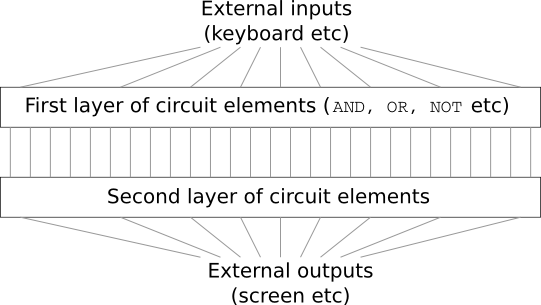
\includegraphics[width=0.7\linewidth]{figures/ch5/shallow_circuit}
\end{center}
You're dumbfounded, and tell your boss: ``The customer is crazy!''

Your boss replies: ``I think they're crazy, too. But what the customer wants, they get.''

In fact, there's a limited sense in which the customer isn't crazy. Suppose you're allowed to use a special logical gate which lets you \inline{AND} together as many inputs as you want. And you're also allowed a many-input \inline{NAND} gate, that is, a gate which can \inline{AND} multiple inputs and then negate the output. With these special gates it turns out to be possible to compute any function at all using a circuit that's just two layers deep.

But just because something is possible doesn't make it a good idea. In practice, when solving circuit design problems (or most any kind of algorithmic problem), we usually start by figuring out how to solve sub-problems, and then gradually integrate the solutions. In other words, we build up to a solution through multiple layers of abstraction.

For instance, suppose we're designing a logical circuit to multiply two numbers. Chances are we want to build it up out of sub-circuits doing operations like adding two numbers. The sub-circuits for adding two numbers will, in turn, be built up out of sub-sub-circuits for adding two bits. Very roughly speaking our circuit will look like:
\begin{center}
	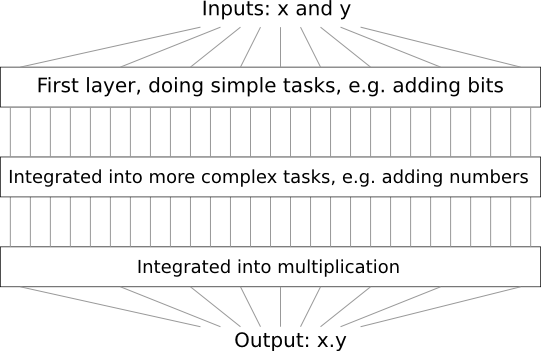
\includegraphics[width=0.7\linewidth]{figures/ch5/circuit_multiplication}
\end{center}
That is, our final circuit contains at least three layers of circuit elements. In fact, it'll probably contain more than three layers, as we break the sub-tasks down into smaller units than I've described. But you get the general idea.

So deep circuits make the process of design easier. But they're not just helpful for design. There are, in fact, mathematical proofs showing that for some functions very shallow circuits require exponentially more circuit elements to compute than do deep circuits. For instance, a famous series of papers in the early 1980s\footnote{The history is somewhat complex, so I won't give detailed references. See Johan H\aa{}stad's 2012 paper \href{http://eccc.hpi-web.de/report/2012/137/}{On the correlation of parity and small-depth circuits} for an account of the early history and references.} showed that computing the parity of a set of bits requires exponentially many gates, if done with a shallow circuit. On the other hand, if you use deeper circuits it's easy to compute the parity using a small circuit: you just compute the parity of pairs of bits, then use those results to compute the parity of pairs of pairs of bits, and so on, building up quickly to the overall parity. Deep circuits thus can be intrinsically much more powerful than shallow circuits.

Up to now, this book has approached neural networks like the crazy customer. Almost all the networks we've worked with have just a single hidden layer of neurons (plus the input and output layers):
\begin{center}
	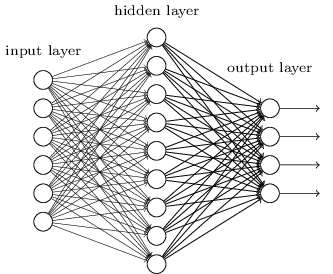
\includegraphics[width=0.6\linewidth]{figures/ch5/tikz35}
\end{center}
These simple networks have been remarkably useful: in earlier chapters we used networks like this to classify handwritten digits with better than 98 percent accuracy! Nonetheless, intuitively we'd expect networks with many more hidden layers to be more powerful:
\begin{center}
	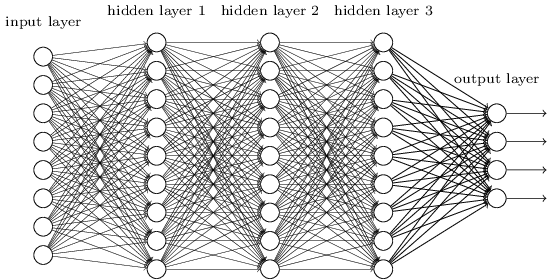
\includegraphics[width=\linewidth]{figures/ch5/tikz36}
\end{center}
Such networks could use the intermediate layers to build up multiple layers of abstraction, just as we do in Boolean circuits. For instance, if we're doing visual pattern recognition, then the neurons in the first layer might learn to recognize edges, the neurons in the second layer could learn to recognize more complex shapes, say triangle or rectangles, built up from edges. The third layer would then recognize still more complex shapes. And so on. These multiple layers of abstraction seem likely to give deep networks a compelling advantage in learning to solve complex pattern recognition problems. Moreover, just as in the case of circuits, there are theoretical results suggesting that deep networks are intrinsically more powerful than shallow networks\footnote{For certain problems and network architectures this is proved in \href{http://arxiv.org/pdf/1312.6098.pdf}{On the number of response regions of deep feed forward networks with piece-wise linear activations}, by Razvan Pascanu, Guido Mont\'ufar, and Yoshua Bengio (2014). See also the more informal discussion in section 2 of \href{http://www.iro.umontreal.ca/~bengioy/papers/ftml_book.pdf}{Learning deep architectures for AI}, by Yoshua Bengio (2009).}.

How can we train such deep networks? In this chapter, we'll try training deep networks using our workhorse learning algorithm -- stochastic gradient descent by backpropagation. But we'll run into trouble, with our deep networks not performing much (if at all) better than shallow networks.

That failure seems surprising in the light of the discussion above. Rather than give up on deep networks, we'll dig down and try to understand what's making our deep networks hard to train. When we look closely, we'll discover that the different layers in our deep network are learning at vastly different speeds. In particular, when later layers in the network are learning well, early layers often get stuck during training, learning almost nothing at all. This stuckness isn't simply due to bad luck. Rather, we'll discover there are fundamental reasons the learning slowdown occurs, connected to our use of gradient-based learning techniques.

As we delve into the problem more deeply, we'll learn that the opposite phenomenon can also occur: the early layers may be learning well, but later layers can become stuck. In fact, we'll find that there's an intrinsic instability associated to learning by gradient descent in deep, many-layer neural networks. This instability tends to result in either the early or the later layers getting stuck during training.

This all sounds like bad news. But by delving into these difficulties, we can begin to gain insight into what's required to train deep networks effectively. And so these investigations are good preparation for the next chapter, where we'll use deep learning to attack image recognition problems.

\section{The vanishing gradient problem}
So, what goes wrong when we try to train a deep network?

To answer that question, let's first revisit the case of a network with just a single hidden layer. As per usual, we'll use the MNIST digit classification problem as our playground for learning and experimentation\footnote{I introduced the MNIST problem and data here\ref{sec:1.5} and here\ref{sec:1.7}.}.

If you wish, you can follow along by training networks on your computer. It is also, of course, fine to just read along. If you do wish to follow live, then you'll need Python 2.7, Numpy, and a copy of the code, which you can get by cloning the relevant repository from the command line:

\begin{lstlisting}
git clone https://github.com/mnielsen/neural-networks-and-deep-learning.git
\end{lstlisting}
If you don't use git then you can download the data and code \href{https://github.com/mnielsen/neural-networks-and-deep-learning/archive/master.zip}{here}. You'll need to change into the \inline{src} subdirectory.
Then, from a Python shell we load the MNIST data:

\begin{lstlisting}
>>> import mnist_loader
>>> training_data, validation_data, test_data = \
... mnist_loader.load_data_wrapper()
\end{lstlisting}
We set up our network:

\begin{lstlisting}
>>> import network2
>>> net = network2.Network([784, 30, 10])
\end{lstlisting}
This network has 784 neurons in the input layer, corresponding to the $28\times28=784$ pixels in the input image. We use 30 hidden neurons, as well as 10 output neurons, corresponding to the 10 possible classifications for the MNIST digits (`0', `1', `2',..., `9').

Let's try training our network for 30 complete epochs, using mini-batches of 10 training examples at a time, a learning rate $\eta=0.1$, and regularization parameter $\lambda=5.0$. As we train we'll monitor the classification accuracy on the \inline{validation_data}\footnote{Note that the networks is likely to take some minutes to train, depending on the speed of your machine. So if you're running the code you may wish to continue reading and return later, not wait for the code to finish executing.}:
\begin{lstlisting}
>>> net.SGD(training_data, 30, 10, 0.1, lmbda=5.0, 
... evaluation_data=validation_data, monitor_evaluation_accuracy=True)
\end{lstlisting}
We get a classification accuracy of 96.48 percent (or thereabouts -- it'll vary a bit from run to run), comparable to our earlier results with a similar configuration.

Now, let's add another hidden layer, also with 30 neurons in it, and try training with the same hyper-parameters:

\begin{lstlisting}
>>> net = network2.Network([784, 30, 30, 10])
>>> net.SGD(training_data, 30, 10, 0.1, lmbda=5.0, 
... evaluation_data=validation_data, monitor_evaluation_accuracy=True)
\end{lstlisting}
This gives an improved classification accuracy, 96.90 percent. That's encouraging: a little more depth is helping. Let's add another 30-neuron hidden layer:

\begin{lstlisting}
>>> net = network2.Network([784, 30, 30, 30, 10])
>>> net.SGD(training_data, 30, 10, 0.1, lmbda=5.0, 
... evaluation_data=validation_data, monitor_evaluation_accuracy=True)
\end{lstlisting}
That doesn't help at all. In fact, the result drops back down to 96.57 percent, close to our original shallow network. And suppose we insert one further hidden layer:

\begin{lstlisting}
>>> net = network2.Network([784, 30, 30, 30, 30, 10])
>>> net.SGD(training_data, 30, 10, 0.1, lmbda=5.0, 
... evaluation_data=validation_data, monitor_evaluation_accuracy=True)
\end{lstlisting}
The classification accuracy drops again, to 96.53 percent. That's probably not a statistically significant drop, but it's not encouraging, either.

This behaviour seems strange. Intuitively, extra hidden layers ought to make the network able to learn more complex classification functions, and thus do a better job classifying. Certainly, things shouldn't get worse, since the extra layers can, in the worst case, simply do nothing\footnote{See this later problem\ref{sec:5.2.1} to understand how to build a hidden layer that does nothing.}. But that's not what's going on.

So what is going on? Let's assume that the extra hidden layers really could help in principle, and the problem is that our learning algorithm isn't finding the right weights and biases. We'd like to figure out what's going wrong in our learning algorithm, and how to do better.

To get some insight into what's going wrong, let's visualize how the network learns. Below, I've plotted part of a [784,30,30,10] network, i.e., a network with two hidden layers, each containing 30 hidden neurons. Each neuron in the diagram has a little bar on it, representing how quickly that neuron is changing as the network learns. A big bar means the neuron's weights and bias are changing rapidly, while a small bar means the weights and bias are changing slowly. More precisely, the bars denote the gradient $\partial C/\partial b$ for each neuron, i.e., the rate of change of the cost with respect to the neuron's bias. Back in Chapter 2 we saw that this gradient quantity controlled not just how rapidly the bias changes during learning, but also how rapidly the weights input to the neuron change, too. Don't worry if you don't recall the details: the thing to keep in mind is simply that these bars show how quickly each neuron's weights and bias are changing as the network learns.

To keep the diagram simple, I've shown just the top six neurons in the two hidden layers. I've omitted the input neurons, since they've got no weights or biases to learn. I've also omitted the output neurons, since we're doing layer-wise comparisons, and it makes most sense to compare layers with the same number of neurons. The results are plotted at the very beginning of training, i.e., immediately after the network is initialized. Here they are\footnote{The data plotted is generated using the program \inline{generate_gradient.py}. The same program is also used to generate the results quoted later in this section.}:
\begin{center}
	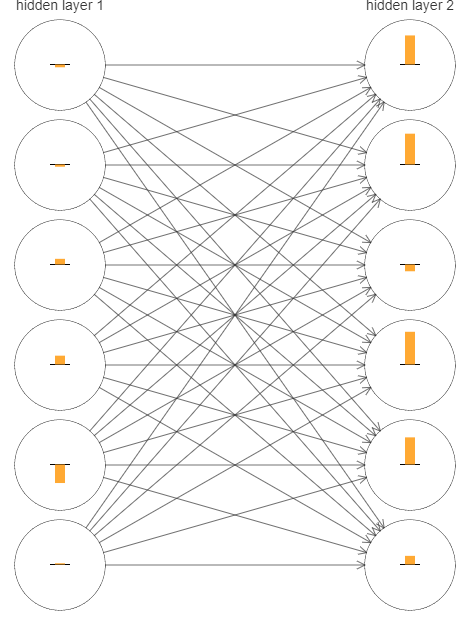
\includegraphics[width=0.45\linewidth]{figures/ch5/tikz500}
\end{center}
The network was initialized randomly, and so it's not surprising that there's a lot of variation in how rapidly the neurons learn. Still, one thing that jumps out is that the bars in the second hidden layer are mostly much larger than the bars in the first hidden layer. As a result, the neurons in the second hidden layer will learn quite a bit faster than the neurons in the first hidden layer. Is this merely a coincidence, or are the neurons in the second hidden layer likely to learn faster than neurons in the first hidden layer in general?

To determine whether this is the case, it helps to have a global way of comparing the speed of learning in the first and second hidden layers. To do this, let's denote the gradient as $\delta^l_j=\partial C/\partial b^l_j$, i.e., the gradient for the $j$-th neuron in the $l$-th layer\footnote{Back in Chapter 2 we referred to this as the error, but here we'll adopt the informal term ``gradient''. I say ``informal'' because of course this doesn't explicitly include the partial derivatives of the cost with respect to the weights, $\partial C/\partial w$.}  We can think of the gradient $\delta^1$ as a vector whose entries determine how quickly the first hidden layer learns, and $\delta^2$ as a vector whose entries determine how quickly the second hidden layer learns. We'll then use the lengths of these vectors as (rough!) global measures of the speed at which the layers are learning. So,for instance, the length $\|\delta^1\|$ measures the speed at which the first hidden layer is learning, while the length $\|\delta^2\|$ measures the speed at which the second hidden layer is learning.

With these definitions, and in the same configuration as was plotted above, we find $\|\delta^1\| = 0.07...$ and $\|\delta^2\|=0.31...$. So this confirms our earlier suspicion: the neurons in the second hidden layer really are learning much faster than the neurons in the first hidden layer.

What happens if we add more hidden layers? If we have three hidden layers, in a [784,30,30,30,10] network, then the respective speeds of learning turn out to be 0.012, 0.060, and 0.283. Again, earlier hidden layers are learning much slower than later hidden layers. Suppose we add yet another layer with 30 hidden neurons. In that case, the respective speeds of learning are 0.003, 0.017, 0.070, and 0.285. The pattern holds: early layers learn slower than later layers.

We've been looking at the speed of learning at the start of training, that is, just after the networks are initialized. How does the speed of learning change as we train our networks? Let's return to look at the network with just two hidden layers. The speed of learning changes as follows:
\begin{center}
	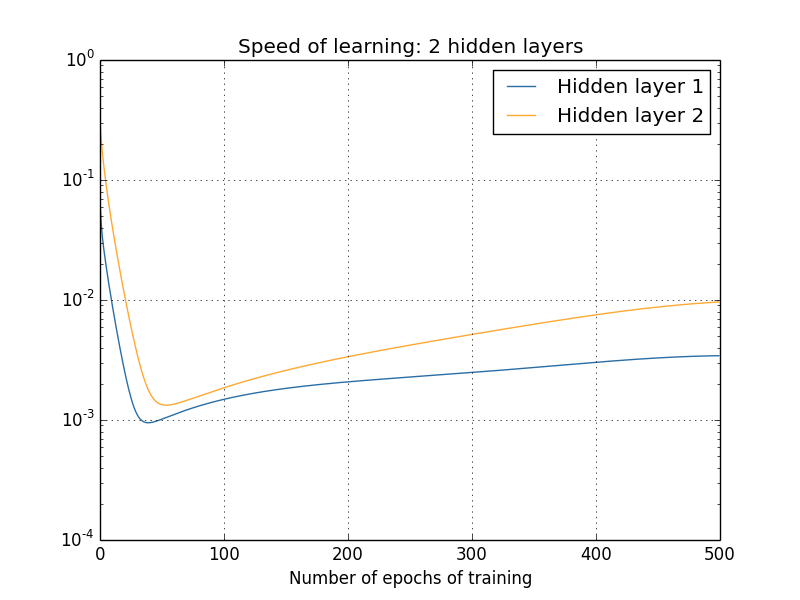
\includegraphics[width=0.7\linewidth]{figures/ch5/training_speed_2_layers}
\end{center}
To generate these results, I used batch gradient descent with just 1,000 training images, trained over 500 epochs. This is a bit different than the way we usually train -- I've used no mini-batches, and just 1,000 training images, rather than the full 50,000 image training set. I'm not trying to do anything sneaky, or pull the wool over your eyes, but it turns out that using mini-batch stochastic gradient descent gives much noisier (albeit very similar, when you average away the noise) results. Using the parameters I've chosen is an easy way of smoothing the results out, so we can see what's going on.

In any case, as you can see the two layers start out learning at very different speeds (as we already know). The speed in both layers then drops very quickly, before rebounding. But through it all, the first hidden layer learns much more slowly than the second hidden layer.

What about more complex networks? Here's the results of a similar experiment, but this time with three hidden layers (a [784,30,30,30,10] network):
\begin{center}
	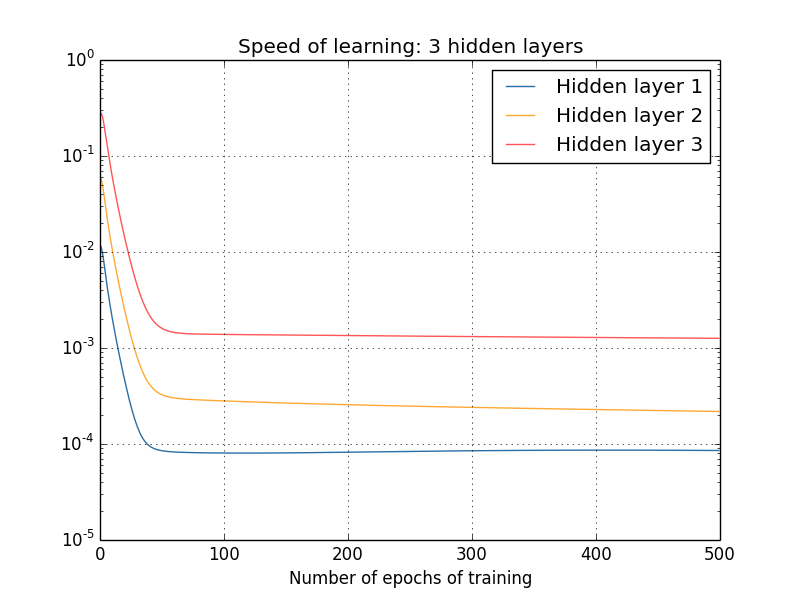
\includegraphics[width=0.7\linewidth]{figures/ch5/training_speed_3_layers}
\end{center}
Again, early hidden layers learn much more slowly than later hidden layers. Finally, let's add a fourth hidden layer (a [784,30,30,30,30,10] network), and see what happens when we train:
\begin{center}
	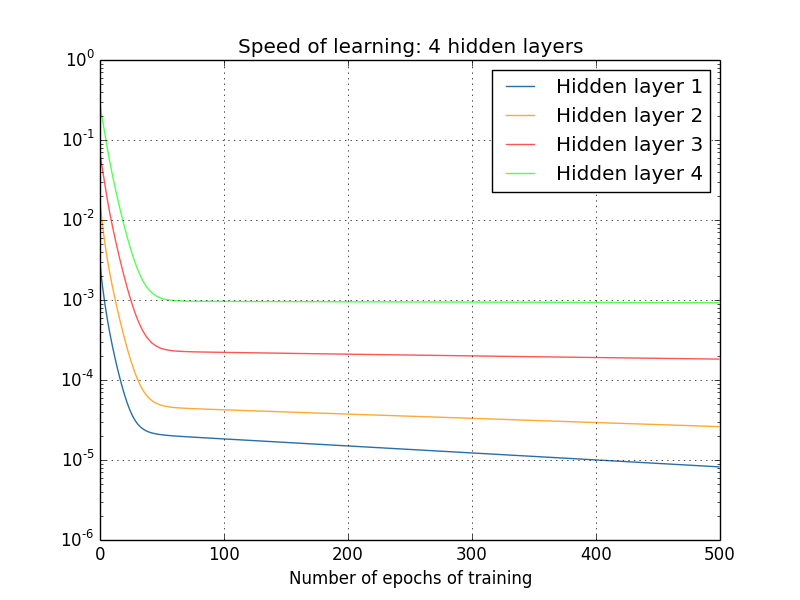
\includegraphics[width=0.7\linewidth]{figures/ch5/training_speed_4_layers}
\end{center}
Again, early hidden layers learn much more slowly than later hidden layers. In this case, the first hidden layer is learning roughly 100 times slower than the final hidden layer. No wonder we were having trouble training these networks earlier!

We have here an important observation: in at least some deep neural networks, the gradient tends to get smaller as we move backward through the hidden layers. This means that neurons in the earlier layers learn much more slowly than neurons in later layers. And while we've seen this in just a single network, there are fundamental reasons why this happens in many neural networks. The phenomenon is known as the vanishing gradient problem\footnote{See \href{http://citeseerx.ist.psu.edu/viewdoc/summary?doi=10.1.1.24.7321}{Gradient flow in recurrent nets: the difficulty of learning long-term dependencies}, by Sepp Hochreiter, Yoshua Bengio, Paolo Frasconi, and J\"urgen Schmidhuber (2001). This paper studied recurrent neural nets, but the essential phenomenon is the same as in the feedforward networks we are studying. See also Sepp Hochreiter's earlier Diploma Thesis, \href{http://www.idsia.ch/~juergen/SeppHochreiter1991ThesisAdvisorSchmidhuber.pdf}{Untersuchungen zu dynamischen neuronalen Netzen} (1991, in German).}.

Why does the vanishing gradient problem occur? Are there ways we can avoid it? And how should we deal with it in training deep neural networks? In fact, we'll learn shortly that it's not inevitable, although the alternative is not very attractive, either: sometimes the gradient gets much larger in earlier layers! This is the exploding gradient problem, and it's not much better news than the vanishing gradient problem. More generally, it turns out that the gradient in deep neural networks is unstable, tending to either explode or vanish in earlier layers. This instability is a fundamental problem for gradient-based learning in deep neural networks. It's something we need to understand, and, if possible, take steps to address.

One response to vanishing (or unstable) gradients is to wonder if they're really such a problem. Momentarily stepping away from neural nets, imagine we were trying to numerically minimize a function $f(x)$ of a single variable. Wouldn't it be good news if the derivative $f'(x)$ was small? Wouldn't that mean we were already near an extremum? In a similar way, might the small gradient in early layers of a deep network mean that we don't need to do much adjustment of the weights and biases?

Of course, this isn't the case. Recall that we randomly initialized the weight and biases in the network. It is extremely unlikely our initial weights and biases will do a good job at whatever it is we want our network to do. To be concrete, consider the first layer of weights in a [784,30,30,30,10] network for the MNIST problem. The random initialization means the first layer throws away most information about the input image. Even if later layers have been extensively trained, they will still find it extremely difficult to identify the input image, simply because they don't have enough information. And so it can't possibly be the case that not much learning needs to be done in the first layer. If we're going to train deep networks, we need to figure out how to address the vanishing gradient problem.

\section{What's causing the vanishing gradient problem? Unstable gradients in deep neural nets}
To get insight into why the vanishing gradient problem occurs, let's consider the simplest deep neural network: one with just a single neuron in each layer. Here's a network with three hidden layers:
\begin{center}
	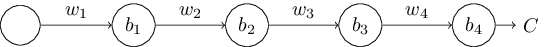
\includegraphics[width=0.7\linewidth]{figures/ch5/tikz37}
\end{center}
Here, $w_1,w_2,\ldots$ are the weights, $b_1,b_2,\ldots$ are the biases, and $C$ is some cost function. Just to remind you how this works, the output $a_j$ from the $j$-th neuron is $\sigma(z_j)$, where $\sigma$ is the usual sigmoid activation function, and $z_j=w_ja_{j-1}+b_j$ is the weighted input to the neuron. I've drawn the cost $C$ at the end to emphasize that the cost is a function of the network's output, $a_4$: if the actual output from the network is close to the desired output, then the cost will be low, while if it's far away, the cost will be high.

We're going to study the gradient $\partial C/\partial b_1$ associated to the first hidden neuron. We'll figure out an expression for $\partial C/\partial b_1$, and by studying that expression we'll understand why the vanishing gradient problem occurs.

I'll start by simply showing you the expression for $\partial C/\partial b_1$. It looks forbidding, but it's actually got a simple structure, which I'll describe in a moment. Here's the expression (ignore the network, for now, and note that $\sigma'$ is just the derivative of the $\sigma$ function):
\begin{center}
	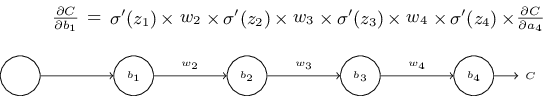
\includegraphics[width=0.7\linewidth]{figures/ch5/tikz38}
\end{center}
The structure in the expression is as follows: there is a $\sigma'(z_j)$ term in the product for each neuron in the network; a weight $w_j$ term for each weight in the network; and a final $\partial C/\partial a_4$ term, corresponding to the cost function at the end. Notice that I've placed each term in the expression above the corresponding part of the network. So the network itself is a mnemonic for the expression.

You're welcome to take this expression for granted, and skip to the discussion of how it relates to the vanishing gradient problem. There's no harm in doing this, since the expression is a special case of our earlier discussion of backpropagation. But there's also a simple explanation of why the expression is true, and so it's fun (and perhaps enlightening) to take a look at that explanation.

Imagine we make a small change $\Delta b_1$ in the bias $b_1$. That will set off a cascading series of changes in the rest of the network. First, it causes a change $\Delta a_1$ in the output from the first hidden neuron. That, in turn, will cause a change $\Delta z_2$ in the weighted input to the second hidden neuron. Then a change $\Delta a_2$ in the output from the second hidden neuron. And so on, all the way through to a change $\Delta C$ in the cost at the output. We have
%$\partial C\partial b1≈\deltaC\delta b_1.(114)
\begin{eqnarray}
\frac{\partial C}{\partial b_1} \approx \frac{\Delta C}{\Delta b_1}.\label{eq:114}
\end{eqnarray}
This suggests that we can figure out an expression for the gradient $\partial C/\partial b_1$ by carefully tracking the effect of each step in this cascade.

To do this, let's think about how $\Delta b_1$ causes the output $a_1$ from the first hidden neuron to change. We have $a_1=\sigma(z_1)=\sigma(w_1a_0+b_1)$, so
%\delta a_1≈=\partial \sigma(w1a0+b1)\partial b1\delta b_1\sigma'(z1)\delta b_1.(115)(116)
\begin{eqnarray}
\Delta a_1 \approx \frac{\partial \sigma(w_1 a_0+b_1)}{\partial b_1} \Delta b_1 = \sigma'(z_1) \Delta b_1. \label{eq:116}
\end{eqnarray}

That $\sigma'(z_1)$ term should look familiar: it's the first term in our claimed expression for the gradient $\partial C/\partial b_1$. Intuitively, this term converts a change $\Delta b_1$ in the bias into a change $\Delta a_1$ in the output activation. That change $\Delta a_1$ in turn causes a change in the weighted input $z_2=w_2a_1+b_2$ to the second hidden neuron:
\begin{eqnarray}
\Delta z_2  \approx \frac{\partial z_2}{\partial a_1} \Delta a_1 =  w_2 \Delta a_1. \label{eq:118}
\end{eqnarray}
Combining our expressions for $\Delta z_2$ and $\Delta a_1$, we see how the change in the bias $b_1$ propagates along the network to affect $z_2$:
\begin{eqnarray}
\Delta z_2 \approx \sigma'(z_1) w_2 \Delta b_1.\label{eq:119}
\end{eqnarray}
%\delta z_2≈\sigma'(z1)w2\delta b_1.(119)
Again, that should look familiar: we've now got the first two terms in our claimed expression for the gradient $\partial C/\partial b_1$.

We can keep going in this fashion, tracking the way changes propagate through the rest of the network. At each neuron we pick up a $\sigma'(z_j)$ term, and through each weight we pick up a $w_j$ term. The end result is an expression relating the final change $\Delta C$ in cost to the initial change $\Delta b_1$ in the bias:
\begin{eqnarray}
\Delta C  \approx  \sigma'(z_1) w_2 \sigma'(z_2) \ldots \sigma'(z_4) \frac{\partial C}{\partial a_4} \Delta b_1. \label{eq:120}
\end{eqnarray}
%\deltaC≈\sigma'(z1)w2\sigma'(z2)…\sigma'(z4)\partial C\partial a4\delta b_1.(120)
Dividing by $\Delta b_1$ we do indeed get the desired expression for the gradient:
%\partial C\partial b1=\sigma'(z1)w2\sigma'(z2)…\sigma'(z4)\partial C\partial a4.(121)
\begin{eqnarray}
\frac{\partial C}{\partial b_1} = \sigma'(z_1) w_2 \sigma'(z_2) \ldots \sigma'(z_4) \frac{\partial C}{\partial a_4}. \label{eq:121}
\end{eqnarray}

\textbf{Why the vanishing gradient problem occurs:} To understand why the vanishing gradient problem occurs, let's explicitly write out the entire expression for the gradient:
\begin{eqnarray}
\frac{\partial C}{\partial b_1} = \sigma'(z_1) \, w_2 \sigma'(z_2) \,w_3 \sigma'(z_3) \, w_4 \sigma'(z_4) \, \frac{\partial C}{\partial a_4}.\label{eq:122}
\end{eqnarray}
Excepting the very last term, this expression is a product of terms of the form $w_j\sigma'(z_j)$. To understand how each of those terms behave, let's look at a plot of the function $\sigma'$:
\begin{center} 
\begin{tikzpicture}
\begin{axis}[title={Derivative of sigmoid function},axis x line=bottom,axis y line=left,width=0.75\linewidth,height=0.35\linewidth,ymin=0,ymax=0.27,scaled y ticks = false,y tick label style={/pgf/number format/fixed},xmin=-5.5,xmax=5.5]
\addplot[blue,domain=-5:5,samples=101]{exp(-x)/(1+exp(-x))/(1+exp(-x))};
\end{axis}
\end{tikzpicture}
\end{center}%
The derivative reaches a maximum at $\sigma'(0)=1/4$. Now, if we use our standard approach to initializing the weights in the network, then we'll choose the weights using a Gaussian with mean 0 and standard deviation 1. So the weights will usually satisfy $|w_j|<1$. Putting these observations together, we see that the terms $w_j\sigma'(z_j)$ will usually satisfy $|w_j\sigma'(z_j)|<1/4$. And when we take a product of many such terms, the product will tend to exponentially decrease: the more terms, the smaller the product will be. This is starting to smell like a possible explanation for the vanishing gradient problem.


To make this all a bit more explicit, let's compare the expression for $\partial C/\partial b_1$ to an expression for the gradient with respect to a later bias, say $\partial C/\partial b_3$. Of course, we haven't explicitly worked out an expression for $\partial C/\partial b_3$, but it follows the same pattern described above for $\partial C/\partial b_1$. Here's the comparison of the two expressions:
\begin{center}
	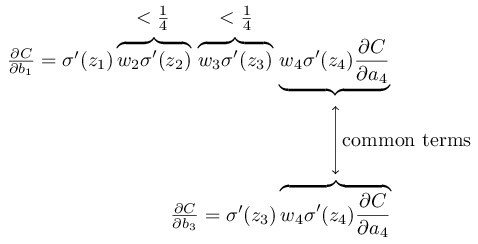
\includegraphics[width=0.7\linewidth]{figures/ch5/tikz39}
\end{center}
The two expressions share many terms. But the gradient $\partial C/\partial b_1$ includes two extra terms each of the form $w_j\sigma'(z_j)$. As we've seen, such terms are typically less than 1/4 in magnitude. And so the gradient $\partial C/\partial b_1$ will usually be a factor of 16 (or more) smaller than $\partial C/\partial b_3$. This is the essential origin of the vanishing gradient problem.

Of course, this is an informal argument, not a rigorous proof that the vanishing gradient problem will occur. There are several possible escape clauses. In particular, we might wonder whether the weights $w_j$ could grow during training. If they do, it's possible the terms $w_j\sigma'(z_j)$ in the product will no longer satisfy $|w_j\sigma'(z_j)|<1/4$. Indeed, if the terms get large enough -- greater than 1 -- then we will no longer have a vanishing gradient problem. Instead, the gradient will actually grow exponentially as we move backward through the layers. Instead of a vanishing gradient problem, we'll have an exploding gradient problem.

\textbf{The exploding gradient problem:} Let's look at an explicit example where exploding gradients occur. The example is somewhat contrived: I'm going to fix parameters in the network in just the right way to ensure we get an exploding gradient. But even though the example is contrived, it has the virtue of firmly establishing that exploding gradients aren't merely a hypothetical possibility, they really can happen.

There are two steps to getting an exploding gradient. First, we choose all the weights in the network to be large, say $w_1=w_2=w_3=w_4=100$. Second, we'll choose the biases so that the $\sigma'(z_j)$ terms are not too small. That's actually pretty easy to do: all we need do is choose the biases to ensure that the weighted input to each neuron is $z_j=0$ (and so $\sigma'(z_j)=1/4$). So, for instance, we want $z_1=w_1a_0+b_1=0$. We can achieve this by setting $b_1=-100\times a_0$. We can use the same idea to select the other biases. When we do this, we see that all the terms $w_j\sigma'(z_j)$ are equal to $100\times1/4=25$. With these choices we get an exploding gradient.

\textbf{The unstable gradient problem:} The fundamental problem here isn't so much the vanishing gradient problem or the exploding gradient problem. It's that the gradient in early layers is the product of terms from all the later layers. When there are many layers, that's an intrinsically unstable situation. The only way all layers can learn at close to the same speed is if all those products of terms come close to balancing out. Without some mechanism or underlying reason for that balancing to occur, it's highly unlikely to happen simply by chance. In short, the real problem here is that neural networks suffer from an \textit{unstable gradient problem}. As a result, if we use standard gradient-based learning techniques, different layers in the network will tend to learn at wildly different speeds.

\begin{exercize}{Exercise}
\item In our discussion of the vanishing gradient problem, we made use of the fact that $|\sigma'(z)|<1/4$. Suppose we used a different activation function, one whose derivative could be much larger. Would that help us avoid the unstable gradient problem?
\end{exercize}
\textbf{The prevalence of the vanishing gradient problem:} We've seen that the gradient can either vanish or explode in the early layers of a deep network. In fact, when using sigmoid neurons the gradient will usually vanish. To see why, consider again the expression $|w\sigma'(z)|$. To avoid the vanishing gradient problem we need $|w\sigma'(z)|\geq1$. You might think this could happen easily if $w$ is very large. However, it's more difficult than it looks. The reason is that the $\sigma'(z)$ term also depends on $w$: $\sigma'(z)=\sigma'(wa+b)$, where $a$ is the input activation. So when we make $w$ large, we need to be careful that we're not simultaneously making $\sigma'(wa+b)$ small. That turns out to be a considerable constraint. The reason is that when we make $w$ large we tend to make $wa+b$ very large. Looking at the graph of $\sigma'$ you can see that this puts us off in the ``wings'' of the $\sigma'$ function, where it takes very small values. The only way to avoid this is if the input activation falls within a fairly narrow range of values (this qualitative explanation is made quantitative in the first problem below). Sometimes that will chance to happen. More often, though, it does not happen. And so in the generic case we have vanishing gradients.

\begin{exercize}{Problems}
\item Consider the product $|w\sigma'(wa+b)|$. Suppose $|w\sigma'(wa+b)|\geq1$. (1) Argue that this can only ever occur if $|w|≥\geq4$. (2) Supposing that $|w|\geq4$, consider the set of input activations a for which $|w\sigma'(wa+b)|\geq1$. Show that the set of a satisfying that constraint can range over an interval no greater in width than
\begin{equation}
%	2|w|ln(|w|(1+1-4/|w|--------√)2-1).(123)
	\frac2{|w|}\ln\left(\frac{|w|(1+\sqrt{1-4/|w|})}{2}-1\right).\label{eq:123}
\end{equation}
(3) Show numerically that the above expression bounding the width of the range is greatest at $|w|\approx6.9$, where it takes a value $\approx0.45$. And so even given that everything lines up just perfectly, we still have a fairly narrow range of input activations which can avoid the vanishing gradient problem.
\item \textbf{Identity neuron:}\label{sec:5.2.1} Consider a neuron with a single input, $x$, a corresponding weight, $w_1$, a bias $b$, and a weight $w_2$ on the output. Show that by choosing the weights and bias appropriately, we can ensure $w_2\sigma(w_1x+b)\approx x$ for $x\in[0,1]$. Such a neuron can thus be used as a kind of identity neuron, that is, a neuron whose output is the same (up to rescaling by a weight factor) as its input. \textit{Hint: It helps to rewrite $x=1/2+\Delta$, to assume $w_1$ is small, and to use a Taylor series expansion in $w_1\Delta$.}
\end{exercize}
\section{Unstable gradients in more complex networks}
We've been studying toy networks, with just one neuron in each hidden layer. What about more complex deep networks, with many neurons in each hidden layer?
\begin{center}
	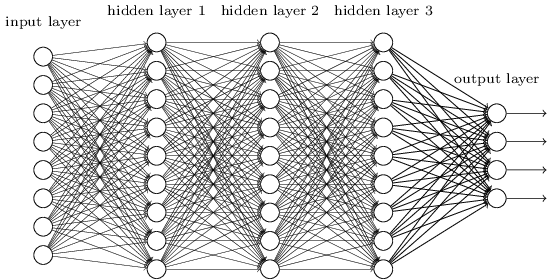
\includegraphics[width=\linewidth]{figures/ch5/tikz40}
\end{center}
In fact, much the same behaviour occurs in such networks. In the earlier chapter on backpropagation we saw that the gradient in the $l$-th layer of an L layer network is given by:

%\deltal=\sigma'(zl)(wl+1)T\sigma'(zl+1)(wl+2)T…\sigma'(zL)∇aC(124)
\begin{eqnarray}
\delta^l = \Sigma'(z^l) (w^{l+1})^T \Sigma'(z^{l+1}) (w^{l+2})^T \ldots\Sigma'(z^L) \nabla_a C
\label{eq:124}
\end{eqnarray}
Here, $\Sigma'(z^l)$ is a diagonal matrix whose entries are the $\sigma'(z)$ values for the weighted inputs to the $l$-th layer. The $w^l$ are the weight matrices for the different layers. And $\nabla_aC$ is the vector of partial derivatives of $C$ with respect to the output activations.

This is a much more complicated expression than in the single-neuron case. Still, if you look closely, the essential form is very similar, with lots of pairs of the form $(w^j)^T\Sigma'(z^j)$. What's more, the matrices $\Sigma'(z^j)$ have small entries on the diagonal, none larger than 1/4. Provided the weight matrices $w^j$ aren't too large, each additional term $(w^j)^T\Sigma'(z^l)$ tends to make the gradient vector smaller, leading to a vanishing gradient. More generally, the large number of terms in the product tends to lead to an unstable gradient, just as in our earlier example. In practice, empirically it is typically found in sigmoid networks that gradients vanish exponentially quickly in earlier layers. As a result, learning slows down in those layers. This slowdown isn't merely an accident or an inconvenience: it's a fundamental consequence of the approach we're taking to learning.

\section{Other obstacles to deep learning}
In this chapter we've focused on vanishing gradients -- and, more generally, unstable gradients -- as an obstacle to deep learning. In fact, unstable gradients are just one obstacle to deep learning, albeit an important fundamental obstacle. Much ongoing research aims to better understand the challenges that can occur when training deep networks. I won't comprehensively summarize that work here, but just want to briefly mention a couple of papers, to give you the flavor of some of the questions people are asking.

As a first example, in 2010 Glorot and Bengio\footnote{\href{http://jmlr.org/proceedings/papers/v9/glorot10a/glorot10a.pdf}{Understanding the difficulty of training deep feedforward neural networks}, by Xavier Glorot and Yoshua Bengio (2010). See also the earlier discussion of the use of sigmoids in \href{http://yann.lecun.com/exdb/publis/pdf/lecun-98b.pdf}{Efficient BackProp}, by Yann LeCun, L\'eon Bottou, Genevieve Orr and Klaus-Robert M\"uller (1998).} found evidence suggesting that the use of sigmoid activation functions can cause problems training deep networks. In particular, they found evidence that the use of sigmoids will cause the activations in the final hidden layer to saturate near 0 early in training, substantially slowing down learning. They suggested some alternative activation functions, which appear not to suffer as much from this saturation problem.

As a second example, in 2013 Sutskever, Martens, Dahl and Hinton\footnote{\href{http://www.cs.toronto.edu/~hinton/absps/momentum.pdf}{On the importance of initialization and momentum in deep learning}, by Ilya Sutskever, James Martens, George Dahl and Geoffrey Hinton (2013).} studied the impact on deep learning of both the random weight initialization and the momentum schedule in momentum-based stochastic gradient descent. In both cases, making good choices made a substantial difference in the ability to train deep networks.

These examples suggest that ``What makes deep networks hard to train?'' is a complex question. In this chapter, we've focused on the instabilities associated to gradient-based learning in deep networks. The results in the last two paragraphs suggest that there is also a role played by the choice of activation function, the way weights are initialized, and even details of how learning by gradient descent is implemented. And, of course, choice of network architecture and other hyper-parameters is also important. Thus, many factors can play a role in making deep networks hard to train, and understanding all those factors is still a subject of ongoing research. This all seems rather downbeat and pessimism-inducing. But the good news is that in the next chapter we'll turn that around, and develop several approaches to deep learning that to some extent manage to overcome or route around all these challenges.


\end{document}
